% Estas slides tienen que abrirse con el programa pdfpc que soporta videos embebidos
% el comando es: pdfpc -g slides.pdf
% para los videos se requiere ubuntu-restricted-extras
% para la bibliografía se requiere biber y configurar texstudio

%\documentclass[compress,handout]{beamer}
\documentclass[aspectratio=169,compress]{beamer}

% add beamer preamble
% In this preamble should go only package and settings related with beamer

% Theme customization
\setbeamertemplate{itemize item}[rectangle] % configure itemize
\setbeamertemplate{itemize subitem}[circle] % configure itemize
\setbeamertemplate{itemize subsubitem}[triangle] % configure itemize
\setbeamertemplate{navigation symbols}{} % remover simbolos de navegacion de las slides
\usefonttheme[onlymath]{serif} % simbolos matematicos en serif (Como es en latex original)
\setbeamersize{text margin left=3mm,text margin right=3mm} 

\setbeamertemplate{blocks}[rounded] % blocks corners rounded
\setbeamercolor{block body}{bg=blue!12,fg=black} % color of blocks
\setbeamertemplate{caption}{\raggedright\insertcaption\par} % elimina la palabra "Figura" del caption

\usepackage[overridenote]{pdfpc} % requires to download manually pdfpc.sty package from https://www.ctan.org/pkg/pdfpc
% para instalar el pdfpc.sty seguir las instrucciones en https://micropore.wordpress.com/2009/11/28/texhash/

%\setbeameroption{show notes on second screen=right} % visualize slides with notes using beamerpresenter slides.pdf

% HOW TO SHOW ADDITIONAL SLIDES%
\newif\ifadditional % conditional to show additional slides
%\additionaltrue   % uncomment to show additional slides
\additionalfalse % uncomment to show without additional slides

% Reference cite without footnote mark
\newrobustcmd*{\footfullcitenomark}{%
    \AtNextCite{%
        \let\thefootnote\relax
        \let\mkbibfootnote\mkbibfootnotetext}%
    \footfullcite}


% add latex preamble
% para la bibliografía se requiere biber y configurar texstudio

% Latex packages
\usepackage[utf8]{inputenc}
\usepackage[T1]{fontenc} % para copiar acentos en español del pdf y permite acentos en las notas
\usepackage[english]{babel}
\usepackage[per-mode = symbol]{siunitx} % para manejar las unidades
\usepackage{multimedia} % to add videos with \movie command
\usepackage{multirow}
\usepackage{graphicx}
\usepackage{xcolor}
\usepackage{amsmath} % bmatrix
\usepackage[makeroom]{cancel} % \cancel to cancel terms in math equations
\renewcommand{\CancelColor}{\color{red}} % set red color for \cancel command
\usepackage[caption=false]{subfig} % caption = false elimina la palabra "Figura" del caption
\usepackage{import} % para el comando import (se usa para pdf_tex)
\captionsetup[subfigure]{labelformat=empty} % remover el indice del caption de la subfigura
\usepackage{booktabs} % \toprule \midrule \bottomrule
\usepackage[backend=biber]{biblatex} % set biber to format references. Must configure Biber in Texstudio
\usepackage{csquotes} % to remove warning triggered by biblatex and babel
\usepackage{algorithm} % to put captions to the algorithmics environmets
\usepackage{algpseudocode} % to write algorithm
\usepackage{tikz} % to use tikz
\usepackage[export]{adjustbox} %valign in subfloat
\usepackage{colortbl} % to paint cells in a table

% Color commands for annotations
\newcommand\TODO[1]{\textbf{\textcolor{red}{#1}}} %  TODO notes

% Graphic paths
\graphicspath{{./images/}}

% listings configuration for C code
\usepackage{listings} % code
\definecolor{commentgreen}{RGB}{2,112,10}
\definecolor{eminence}{RGB}{108,48,130}
\definecolor{weborange}{RGB}{255,165,0}
\definecolor{frenchplum}{RGB}{129,20,83}

\lstset{ % spanish characters for listings package
	inputencoding=latin1,
    columns=fullflexible,
	breaklines=true,
	tabsize=2,
	showstringspaces=false,
	basicstyle=\ttfamily,
	backgroundcolor=\color{lightgray}, % Choose background color
	literate={á}{{\'a}}1
	{ã}{{\~a}}1
	{é}{{\'e}}1
	{ó}{{\'o}}1
	{í}{{\'i}}1
	{ñ}{{\~n}}1
	{¡}{{!`}}1
	{¿}{{?`}}1
	{ú}{{\'u}}1
	{Í}{{\'I}}1
	{Ó}{{\'O}}1
    {-}{-}1
}

\lstdefinestyle{cpp}{ % spanish characters for listings package
    language=C++,
   	commentstyle=\color{commentgreen},
    keywordstyle=\color{eminence},
    stringstyle=\color{red},
    emph={int,char,double,float,unsigned,void,bool},
    emphstyle={\color{blue}}
}

\lstdefinestyle{bash}{ % spanish characters for listings package
	language=Bash
}

\lstdefinestyle{xml}{
	language=XML,
	morekeywords={encoding,xs:schema,xs:element,xs:complexType,xs:sequence,xs:attribute}
}

\lstdefinestyle{cmake}{
	language=make, % there is no cmake support in listings
}

\lstdefinestyle{python}{
    language=python,
}


%%%%% PARA QUE EN LAS TABLAS SE PUEDA PONER UN SALTO DE LINEA DENTRO DE UNA CELDA
\newcommand{\specialcell}[2][c]{%
    \begin{tiny}
        \begin{tabular}[#1]{@{}c@{}}#2\end{tabular}  
    \end{tiny}
}
%%%%%%%%%%%%%%%%%%%%%%%%%%%%%%%%%%%%%%%%%%%%%%%%%%%%%%%%%%%%%%%%%%%%%%%%

%%%%% PARA QUE LAS TABLAS TENGAN TODAS LAS COLUMNAS CENTRADAS Y DE IGUAL TAMAÑO
\usepackage{tabularx}
\renewcommand{\tabularxcolumn}[1]{>{\centering\arraybackslash}m{#1}}
%%%%%%%%%%%%%%%%%%%%%%%%%%%%%%%%%%%%%%%%%%%%%%%%%%%%%%%%%%%%%%%%%%%%%%%%



% add math preamble
\usepackage{amsmath}
\usepackage{amssymb}
\usepackage{amsopn}
\usepackage{mathtools}

% set matrix maximum length
\setcounter{MaxMatrixCols}{20}

% math
\renewcommand{\vec}[1]{\boldsymbol{\mathbf{#1}}}
\newcommand{\norm}[1]{\lVert#1\rVert}

% Declare arg max and arg min functionss
\DeclareMathOperator*{\argmax}{arg\,max}
\DeclareMathOperator*{\argmin}{arg\,min}

% Declare atan2 
\DeclareMathOperator{\atantwo}{atan2}

% Homogeneous decoration function
\newcommand{\homo}[1]{\dot{#1}}


% Declare projection as math function
\DeclareMathOperator{\proj}{proj}
\newcommand{\fromCoord}[2]{{#1}_\mathrm{#2}}
\newcommand{\toCoord}[2]{\prescript{\mathrm{#2}}{}{#1}}
\newcommand{\worldCoordSystem}{\mathrm{W}}
\newcommand{\bodyCoordSystem}{\mathrm{B}}
\newcommand{\cameraCoordSystem}{\mathrm{C}}
\newcommand{\origin}{\vec{o}}
\newcommand{\point}{\vec{p}}
\newcommand{\worldPoint}{\toCoord{\point}{\worldCoordSystem}}
\newcommand{\imagePoint}{\vec{u}}
\newcommand{\cameraPoint}{\toCoord{\point}{\cameraCoordSystem}}
\newcommand{\homoWorldPoint}{\toCoord{\homo{\point}}{\worldCoordSystem}}
\newcommand{\homoImagePoint}{\homo{\imagePoint}}
\newcommand{\homoCameraPoint}{\toCoord{\homo{\point}}{\cameraCoordSystem}}
\newcommand{\measurement}{\vec{z}}
\newcommand{\prediction}{\hat{\vec{z}}}
\newcommand{\seMatrix}{\vec{\xi}}
\newcommand{\transform}[2]{\toCoord{\fromCoord{\seMatrix}{#2}}{#1}}
\newcommand{\pointCoord}[1]{\toCoord{\point}{#1}}
\newcommand{\rotation}{\vec{R}}
\newcommand{\rotationCoord}[2]{\toCoord{\fromCoord{\rotation}{#2}}{#1}}
\newcommand{\translation}{\vec{t}}
\newcommand{\translationCoord}[2]{\toCoord{\fromCoord{\translation}{#2}}{#1}}
\newcommand{\intrinsicMatrix}{\vec{K}}
\newcommand{\principalPoint}{\vec{c}}
\newcommand{\reprojectionError}{u}
\newcommand{\projectionMatrix}{\vec{P}}
\newcommand{\cameraCenter}{\vec{o}}
\newcommand{\worldCameraCenter}{\toCoord{\cameraCenter}{\worldCoordSystem}}
\newcommand{\essentialMatrix}{\vec{E}}
\newcommand{\fundamentalMatrix}{\vec{F}}
\newcommand{\inverse}[1]{{#1}^{-1}}
\newcommand{\epipole}{\vec{e}}

% Localization (State Estimation)
\newcommand{\state}{x}
\newcommand{\observation}{z}
\newcommand{\controlCommand}{u}
\newcommand{\covariance}{\Sigma}
\newcommand{\motionModelNoise}{\epsilon}
\newcommand{\measurementModelNoise}{\delta}
\newcommand{\motionModelFunction}[1]{g\left( #1 \right)}
\newcommand{\observationModelFunction}[1]{h\left( #1 \right)}
\newcommand{\motionParametersCovariance}{R}
\newcommand{\observationModelCovariance}{Q}
\newcommand{\motionModelJacobian}{G}
\newcommand{\observationModelJacobian}{H}
\newcommand{\kalmanGain}{K}
\newcommand{\normalDistribution}[2]{\mathcal{N}\left( {#1}, {#2} \right)}
\newcommand{\motionModelJacobianControl}{V}
\newcommand{\motionModelCovariance}{M}
\newcommand{\stateEvolutionMatrix}{A}

% Mapping slides
\newcommand{\map}{m}
\newcommand{\mapRandomVariable}{m}

% SLAM slides
\newcommand{\informationMatrix}{\vec{\Omega}}
\newcommand{\error}{\vec{e}}
\newcommand{\observationBold}{\vec{z}}
\newcommand{\stateBold}{\vec{x}}
\newcommand{\jacobian}{\vec{J}}
\newcommand{\linearSystemb}{\vec{b}}
\newcommand{\linearSystemH}{\vec{H}}


% Motion Planning slides
\newcommand{\workSpace}{\mathcal{W}}
\newcommand{\obstaclesSet}{\mathcal{O}}
\newcommand{\robotInConfiguration}{\mathcal{A}}
\newcommand{\robotConfiguration}{q}
\newcommand{\configurationSpace}{\mathcal{C}}
\newcommand{\freeConfigurationSpace}{\configurationSpace_{free}}
\newcommand{\obstableConfigurationSpace}{\configurationSpace_{obs}}
\newcommand{\goalSet}{\configurationSpace_{goal}}
\newcommand{\startConfiguration}{\robotConfiguration_{I}}
\newcommand{\goalConfiguration}{\robotConfiguration_{G}}
\newcommand{\continuousPath}{\tau}
\newcommand{\motionLaw}{\gamma}
\newcommand{\robotActionSpace}{\mathcal{U}}


% Motion model
\newcommand{\position}{\vec{p}}
\newcommand{\orientation}{\vec{O}}
\newcommand{\orientationQuaternion}{\vec{q}}
\newcommand{\predictedPosition}{\hat{\vec{p}}}
\newcommand{\predictedOrientationQuaternion}{\hat{\vec{q}}}
\newcommand{\linearVelocity}{\vec{v}}
\newcommand{\angularVelocity}{\vec{\omega}}

\DeclareMathOperator{\slerpOp}{slerp}
\newcommand{\slerp}[1]{\slerpOp{\left( #1 \right)}}

% Map structure
\newcommand{\keyframesSet}{K}
\newcommand{\mapPointsSet}{P}
\newcommand{\observedMapPoints}{O}
\newcommand{\covisibilityKeyframes}{CK}
\newcommand{\localMap}{local\_map}

% Bundle Adjutment
\newcommand{\update}{\vec{\delta}}
\newcommand{\incremental}{\hat{\update}}


% Loop Closure names

% scaled operators and letters to fancy view
\newcommand{\sminus}{\scalebox{0.5}[1.0]{$-$}}
\newcommand{\splus}{\scalebox{0.6}[0.6]{$+$}}
\newcommand{\curr}{c}
\newcommand{\sind}[1]{\scalebox{0.6}[0.6]{$#1$}}
\newcommand{\ind}[1]{\scalebox{0.7}[0.7]{$#1$}}

\newcommand{\keyframe}{\vec{K}}
\newcommand{\bowVector}{\vec{v}}
\newcommand{\lcError}{\vec{\Omega}}
\newcommand{\relativeTransformation}{\seMatrix}
\DeclareMathOperator{\interpolate}{interpolate}

\newcommand{\relativeMotion}{\vec{\delta}}
\newcommand{\groundTruth}[1]{{#1}^{*}}

% definición del operador rot()
\DeclareMathOperator{\rotationOp}{rot}
\newcommand{\getRotation}[1]{\rotationOp{\left( #1 \right)}}

\DeclareMathOperator{\translationOp}{trans}
\newcommand{\getTranslation}[1]{\translationOp{\left( #1 \right)}}









% add bibliography resource
\renewcommand*{\bibfont}{\footnotesize} % change bibliograhy size
\bibliography{../../common/bibliography.bib}

\subtitle{Localization}
\title{Mobile Robotics}
\author{Taihú Pire}
\institute{Robotics Laboratory}
\titlegraphic{
\includegraphics[width=0.4\textwidth]{images/cifasis_logo.pdf}}
\date{}


\begin{document}

 % add title page
 \frame{\titlepage}

 \section{Bayes filter}
 \begin{frame}
    \frametitle{Topics of these slides}
    
    \begin{itemize}
        \item Bayes filter
        \item Kalman filter
        \item Extended Kalman filter (EKF)
        \item Particle filter
    \end{itemize}
    
\end{frame}
    
\begin{frame}
    \frametitle{Localization}
    \begin{block}{Localization}
        It is the ability of a machine (robot) to locate itself in space.
    \end{block}
\end{frame}
    
\begin{frame}
    \frametitle{State Estimation}
    
    \note{Information obtained from Cyrill Stachniss Bayes: https://youtu.be/0lKHFJpaZvE}
    
    \begin{itemize}
        \item Estimate the \textbf{state} $\state$ of a system given the \textbf{observations} $\observation$ and \textbf{control commands} $\controlCommand$
        \item Objective:
    \end{itemize}
    
    \begin{equation}
        p\left(\state_{t} | \observation_{1:t}, \controlCommand_{1:t} \right)
    \end{equation}
    
    Recursive State Estimation: This involves estimating the current state $\state_{t}$ using the immediately preceding state $\state_{t-1}$ as well. \end{frame}
    
    \begin{frame}{Recursive Bayes Filter}
    \begin{block}{Example}
        \begin{itemize}
            \item Given a robot in a one-dimensional world, with no knowledge of where it is
            \item The robot can move forward or backward
            \item Suppose further that there are three doors (\alert{landmarks}), the robot can detect whether it is next to a door or not.
        \end{itemize}
    \end{block}
    
    \begin{center}
        \includegraphics<1>[width=0.7\columnwidth]{./images/monte_carlo_example.pdf}
    \end{center}
    
\end{frame}
    
\begin{frame}
    \frametitle{Recursive Bayes Filter: Initial Position}
    Since the robot initially does not know its position, it is equally possible that it is located anywhere in the world (\alert{belief}). We can represent this mathematically by saying that the robot's \alert{probability distribution function} is \alert{uniform} over the world it is in.
    \begin{center}
        \includegraphics<1>[width=0.7\columnwidth]{./images/monte_carlo_uniform.pdf}
    \end{center}
    
\end{frame}
    
\begin{frame}
    \frametitle{Recursive Bayes Filter: Measurement}
    
    If the robot senses that it is next to a door, then its belief about its location is altered as follows:
    
    \begin{center}
        \includegraphics<1>[width=0.7\columnwidth]{./images/monte_carlo_sensing.pdf}
    \end{center}
    
    This new function represents another probability distribution called \alert{Posterior belief}.
    
    The Posterior belief function is the best representation of the robot's current position. Each hill represents the evaluation of its position relative to a door.
    
    The probability $p(\measurement | \state)$ reads: ``Given that we know where the robot is, what is the probability of observing the door?''
    
\end{frame}
    
\begin{frame}
    \frametitle{Recursive Bayes Filter: Movement}
    
    If \textbf{the robot moves to the right}, the belief changes according to the movement.
    
    Just as the robot's movement is inaccurate, its uncertainty increases as it moves; in other words, the hills are flattened. This flattening is mathematically carried out through the \alert{convolution} operation between the Posterior belief function and the function that describes the distance traveled.
    
    \begin{center}
        \includegraphics<1>[width=0.7\columnwidth]{./images/monte_carlo_moving.pdf}
    \end{center}
    
    The convolution operation measures the overlap as one function slides over another.
    
\end{frame}
    
\begin{frame}
    \frametitle{Recursive Bayes Filter: Second Measurement}
    Suppose the robot, after moving, senses that it is next to a door again. Then, as before, the probability where there is a door will increase by a certain factor of the probability function.
    
    \begin{center}
        \includegraphics<1>[width=0.7\columnwidth]{./images/monte_carlo_sensing2.pdf}
    \end{center}
\end{frame}
    
\begin{frame}
    \frametitle{Recursive Bayes Filter: Second Movement}
    Suppose the robot moves again...
    
    \begin{center}
        \includegraphics<1>[width=0.7\columnwidth]{./images/monte_carlo_moving2.pdf}
    \end{center}
\end{frame}


\begin{frame}
    \frametitle{State Estimation}
    
    \note{Information obtained from Cyrill Stachniss Bayes: https://youtu.be/0lKHFJpaZvE}
    
    \begin{itemize}
        \item Estimate the state $\state$ of a system given the observations $\observation$ and control commands $\controlCommand$
    \item Objective:
    \end{itemize}
    
    \begin{equation}
        p\left(\state_{t} | \observation_{1:t}, \controlCommand_{1:t} \right)
    \end{equation}
    
    Recursive state estimation: This involves estimating the current state $\state_{t}$ using the immediately preceding state $\state_{t-1}$ as well.
\end{frame}
    
\begin{frame}
    \frametitle{State Estimation}
    
    \note{Information obtained from Cyrill Stachniss Bayes: https://youtu.be/0lKHFJpaZvE}
    We are interested in the system's belief (\emph{belief}) about where it is at time $t$:
    
    \begin{equation*}
    bel(\state_{t}) = p\left(\state_{t} | \observation_{1:t}, \controlCommand_{1:t} \right) \quad \text{\scriptsize (state estimation equation or probability distribution definition)}
    \end{equation*}
    
    The equation can be read as: ``Where am I now $\state_{t}$, given all observations $\observation_{1:t}$ and all control commands $\controlCommand_{1:t}$''
    
    \vspace{1cm}
    
    Now let's simplify the distribution using Bayes' Rule:
    
\end{frame}


\begin{frame}
    \frametitle{Derivación del Filtro de Bayes Recursivo}
    
    \note{Información obtenida de Cyrill Stachniss Bayes: https://youtu.be/0lKHFJpaZvE}
    $\begin{aligned}
        \only<1>{
            bel(\state_{t}) &= p\left(\state_{t} | \observation_{1:t}, \controlCommand_{1:t} \right)\\
                }
        \only<2>{
            bel(\state_{t}) &= \alert{p\left(\state_{t} | \observation_{1:t}, \controlCommand_{1:t} \right)}\\
                            &= \eta \, p\left(\observation_{t} |\state_{t}, \observation_{1:t-1}, \controlCommand_{1:t} \right) p\left(\state_{t} | \observation_{1:t-1}, \controlCommand_{1:t} \right) \quad \text{where $\eta$ is a normalization constant}\\
                }
        \only<3>{
            bel(\state_{t}) &= p\left(\state_{t} | \observation_{1:t}, \controlCommand_{1:t} \right)\\
                            &= \eta \, \alert{p\left(\observation_{t} |\state_{t}, \observation_{1:t-1}, \controlCommand_{1:t} \right)} p\left(\state_{t} | \observation_{1:t-1}, \controlCommand_{1:t} \right) \quad \text{where $\eta$ is a normalization constant}\\
                            &= \eta \, p\left(\observation_{t} |\state_{t} \right) p\left(\state_{t} | \observation_{1:t-1}, \controlCommand_{1:t} \right)\\
                }
        \only<4>{
            bel(\state_{t}) &= p\left(\state_{t} | \observation_{1:t}, \controlCommand_{1:t} \right)\\
                            &= \eta \, p\left(\observation_{t} |\state_{t}, \observation_{1:t-1}, \controlCommand_{1:t} \right) p\left(\state_{t} | \observation_{1:t-1}, \controlCommand_{1:t} \right) \quad \text{where $\eta$ is a normalization constant}\\
                            &= \eta \, p\left(\observation_{t} |\state_{t} \right) \alert{p\left(\state_{t} | \observation_{1:t-1}, \controlCommand_{1:t} \right)}\\
                            &= \eta \, p\left(\observation_{t} |\state_{t} \right) \int p\left(\state_{t} | \state_{t-1}, \observation_{1:t-1}, \controlCommand_{1:t} \right) p\left(\state_{t-1} | \observation_{1:t-1}, \controlCommand_{1:t} \right) d \state_{t-1}\\
                }
        \only<5>{
            bel(\state_{t}) &= p\left(\state_{t} | \observation_{1:t}, \controlCommand_{1:t} \right)\\
                            &= \eta \, p\left(\observation_{t} |\state_{t}, \observation_{1:t-1}, \controlCommand_{1:t} \right) p\left(\state_{t} | \observation_{1:t-1}, \controlCommand_{1:t} \right) \quad \text{where $\eta$ is a normalization constant}\\
                            &= \eta \, p\left(\observation_{t} |\state_{t} \right) p\left(\state_{t} | \observation_{1:t-1}, \controlCommand_{1:t} \right)\\
                            &= \eta \, p\left(\observation_{t} |\state_{t} \right) \int \alert{p\left(\state_{t} | \state_{t-1}, \observation_{1:t-1}, \controlCommand_{1:t} \right)} p\left(\state_{t-1} | \observation_{1:t-1}, \controlCommand_{1:t} \right) d \state_{t-1}\\
                            &= \eta \, p\left(\observation_{t} |\state_{t} \right) \int p\left(\state_{t} | \state_{t-1}, \controlCommand_{t} \right) p\left(\state_{t-1} | \observation_{1:t-1}, \controlCommand_{1:t} \right) d \state_{t-1}\\
                }
        \only<6>{
            bel(\state_{t}) &= p\left(\state_{t} | \observation_{1:t}, \controlCommand_{1:t} \right)\\
                            &= \eta \, p\left(\observation_{t} |\state_{t}, \observation_{1:t-1}, \controlCommand_{1:t} \right) p\left(\state_{t} | \observation_{1:t-1}, \controlCommand_{1:t} \right) \quad \text{where $\eta$ is a normalization constant}\\
                            &= \eta \, p\left(\observation_{t} |\state_{t} \right) p\left(\state_{t} | \observation_{1:t-1}, \controlCommand_{1:t} \right)\\
                            &= \eta \, p\left(\observation_{t} |\state_{t} \right) \int p\left(\state_{t} | \state_{t-1}, \observation_{1:t-1}, \controlCommand_{1:t} \right) p\left(\state_{t-1} | \observation_{1:t-1}, \controlCommand_{1:t} \right) d \state_{t-1}\\
                            &= \eta \, p\left(\observation_{t} |\state_{t} \right) \int p\left(\state_{t} | \state_{t-1}, \controlCommand_{t} \right) p\left(\state_{t-1} | \observation_{1:t-1}, \alert{\controlCommand_{1:t}} \right) d \state_{t-1}\\
                            &= \eta \, p\left(\observation_{t} |\state_{t} \right) \int p\left(\state_{t} | \state_{t-1}, \controlCommand_{t} \right) p\left(\state_{t-1} | \observation_{1:t-1}, \controlCommand_{1:t-1} \right) d \state_{t-1}\\
                }
        \only<7>{
            bel(\state_{t}) &= p\left(\state_{t} | \observation_{1:t}, \controlCommand_{1:t} \right)\\
                            &= \eta \, p\left(\observation_{t} |\state_{t}, \observation_{1:t-1}, \controlCommand_{1:t} \right) p\left(\state_{t} | \observation_{1:t-1}, \controlCommand_{1:t} \right) \quad \text{where $\eta$ is a normalization constant}\\
                            &= \eta \, p\left(\observation_{t} |\state_{t} \right) p\left(\state_{t} | \observation_{1:t-1}, \controlCommand_{1:t} \right)\\
                            &= \eta \, p\left(\observation_{t} |\state_{t} \right) \int p\left(\state_{t} | \state_{t-1}, \observation_{1:t-1}, \controlCommand_{1:t} \right) p\left(\state_{t-1} | \observation_{1:t-1}, \controlCommand_{1:t} \right) d \state_{t-1}\\
                            &= \eta \, p\left(\observation_{t} |\state_{t} \right) \int p\left(\state_{t} | \state_{t-1}, \controlCommand_{t} \right) p\left(\state_{t-1} | \observation_{1:t-1}, \controlCommand_{1:t} \right) d \state_{t-1}\\
                            &= \eta \, p\left(\observation_{t} |\state_{t} \right) \int p\left(\state_{t} | \state_{t-1}, \controlCommand_{t} \right) \alert{p\left(\state_{t-1} | \observation_{1:t-1}, \controlCommand_{1:t-1} \right)} d \state_{t-1}\\
                            &= \eta \, p\left(\observation_{t} |\state_{t} \right) \int p\left(\state_{t} | \state_{t-1}, \controlCommand_{t} \right) bel(\state_{t-1}) d \state_{t-1}
                }
    \end{aligned}$
    \only<2>{\alert{Bayes' Rule} \note{eta encodes the normalization performed by the divisor term of Bayes' rule.}}
    \only<3>{\alert{Markov assumption. What I measure now $\observation_{t}$ depends only on the current state $\state_{t}$ and is independent of previous measurements $\observation_{1:t-1}$ and all commands $\controlCommand_{1:t}$}}
    \only<4>{\alert{Law of total probability. That is, we integrate over all possible previous states. This can be interpreted as ``Where are we now, given the previous state $\state_{t-1}$ multiplied by how likely it is that said state $\state_{t-1}$ will be reached.''}}
    \only<5>{\alert{Markov assumption. If $\state_{t-1}$ is given, then all measurements $\observation_{1:t-1}$ and commands $\controlCommand_{t-1}$ are irrelevant. We care about $\controlCommand_{t}$ because it tells us how it evolves from $\state_{t-1}$ to $\state_{t}$ }}
    \only<6>{\alert{Independence assumption. We assume that a future command $\controlCommand_{t}$ does not help us know our current state $\state_{t}$.}} \note{We lose information since we assume independence. We assume that a future command does not help us know our current pose. This is not always true. For example, when a robot is very close to a wall, the control system would hardly give a command that makes the robot move towards the wall. Therefore, if we know that the next command from the control system makes us turn or go backward, then we could infer that we are close to the wall.}
    \only<7>{\alert{Recursive term!}}
    \note{Then we can continue to make assumptions, for example, assuming that the probabilities are Gaussian. Which is not true in general.}
\end{frame}

\begin{frame}
    \frametitle{Prediction Step and Correction Step}
    \note{Information obtained from Cyrill Stachniss Bayes: https://youtu.be/0lKHFJpaZvE}
    \begin{itemize}
        \item The Bayes Filter can be written as a two-step process
        \begin{equation*}
        bel(\state_{t}) = \eta \, p\left(\observation_{t} |\state_{t} \right) \int p\left(\state_{t} | \state_{t-1}, \controlCommand_{t} \right) bel(\state_{t-1}) d \state_{t-1}
        \end{equation*}
        \item Prediction Step
        \begin{equation*}
        \overline{bel}(\state_{t}) = \int p\left(\state_{t} | \state_{t-1}, \controlCommand_{t} \right) bel(\state_{t-1}) d \state_{t-1}
        \end{equation*}
        \item Correction Step
        \begin{equation*}
        bel(\state_{t}) = \eta \, p\left(\observation_{t} |\state_{t} \right) \overline{bel}(\state_{t})
        \end{equation*}
    \end{itemize}
    
    \note{The prediction step: predicts where we will be given the control commands}
    \note{The correction step: taking into account the current measurements, corrects the predicted pose}
    
\end{frame}
    
\begin{frame}
    \frametitle{Motion model and observation model}
    \note{Information obtained from Cyrill Stachniss Bayes: https://youtu.be/0lKHFJpaZvE} 
    \begin{itemize}
        \item Prediction Step
        \begin{equation*}
        \overline{bel}(\state_{t}) = \int \underbrace{p\left(\state_{t} | \state_{t-1}, \controlCommand_{t} \right)}_{\text{Motion model}} bel(\state_{t-1}) d \state_{t-1}
        \end{equation*}
        \item Correction Step
        \begin{equation*}
        bel(\state_{t}) = \eta \underbrace{p\left(\observation_{t} |\state_{t} \right)}_{\text{\makebox[0pt]{Observation model (Measurement model or Sensor model)}}} \overline{bel}(\state_{t})
        \end{equation*}
    \end{itemize}
    
    \note{The prediction step: predicts where we will be given the control commands}
    \note{The correction step: taking into account the current measurements, corrects the pose predicted}
    
\end{frame}
    
\begin{frame}
    \frametitle{Different implementations}
    \note{Information obtained from Cyrill Stachniss Bayes: https://youtu.be/0lKHFJpaZvE}
    \begin{itemize}
        \item The Bayes Filter is a recursive state estimation framework
        \item There are different implementations
        \item Different Properties:
        \begin{itemize}
            \item Linear vs. nonlinear models for motion and observation modeling
            \item Using only Gaussian probability distributions?
            \item Parametric and non-parametric filters (represent the probability distribution parametrically or non-parametrically)
            \item ...
        \end{itemize}
    \end{itemize}
\end{frame}
    
\begin{frame}
    \frametitle{Popular filters}
    \note{Information obtained from Cyrill Stachniss Bayes: https://youtu.be/0lKHFJpaZvE}
    \begin{itemize}
        \item Kalman Filter
        \begin{itemize}
            \item Uses Gaussian probability distributions
            \item Only works with linear motion and observation models
        \end{itemize}
        \item Extended Kalman Filter (EKF)
        \begin{itemize}
            \item Uses Gaussian probability distributions
            \item {\bf Linearizes} nonlinear motion and observation models using a Taylor approximation
        \end{itemize} 
        \item Particle filter
        \begin{itemize}
            \item Non-parametric
            \item Models of arbitrary probabilistic distributions, that is, not everything is Gaussian (sample sampling stage)
        \end{itemize}
     \end{itemize}
    
     \note{- Nonparametric filters represent posterior state as a function of previous state.
     - Nonparametric filters does not rely on a fixed functional form of
     later.
     - Histogram filter and Particle filter represent state space and posterior as a finite set of data.
     - There is usually a trade-off between efficiency and level of detail of data.}
     \note{the price to pay is that it has a very high computational cost}
\end{frame}
    
\begin{frame}{Motion Model}
    \note{Information obtained from Cyrill Stachniss Bayes: https://youtu.be/0lKHFJpaZvE}
    \begin{equation*}
    \overline{bel}(\state_{t}) = \int \underbrace{p\left(\state_{t} | \state_{t-1}, \controlCommand_{t} \right)}_{\text{Motion model}} bel(\state_{t-1}) d \state_{t-1}
    \end{equation*}
\end{frame}

\begin{frame}
    \frametitle{Example: Odometry-Based Motion}
    \note{Information obtained from Cyrill Stachniss Bayes: https://youtu.be/0lKHFJpaZvE}
    
    \begin{figure}[!h]
        \centering
        \subfloat[Motion Model Covariance]
        {
        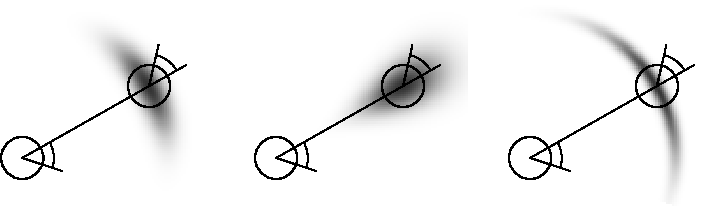
\includegraphics[width=0.6\columnwidth]{./images/covariance_odometry_motion_model.pdf}
        }\\
        \subfloat[Motion Model Samples]
        {
        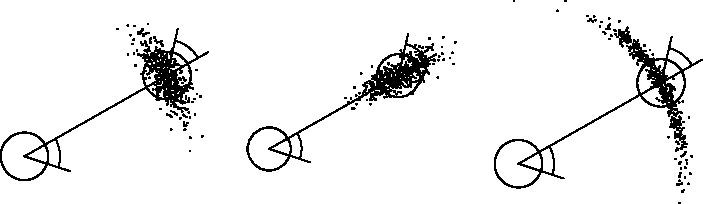
\includegraphics[width=0.6\columnwidth]{./images/sampling_odometry_motion_model.pdf}
        }
    \end{figure}
    
\end{frame}
    
\begin{frame}
    \frametitle{Observation Model}
    \note{Information obtained from Cyrill Stachniss Bayes: https://youtu.be/0lKHFJpaZvE}
    \begin{equation*}
    bel(\state_{t}) = \eta \underbrace{p\left(\observation_{t} |\state_{t} \right)}_{\text{\makebox[0pt]{Observation model (Measurement model or Sensor model)}}} \overline{bel}(\state_{t})
    \end{equation*}
\end{frame}
    
\begin{frame}{Example: Simple Observation Model with Gaussian Noise}
    \note{Information obtained from Cyrill Stachniss Bayes: https://youtu.be/0lKHFJpaZvE}
    
    \begin{itemize}
        \item Range sensor estimating the distance to a nearby object
        \item Gaussian noise in the sensor reading
    \end{itemize} 
    
    \begin{figure}[!h]
        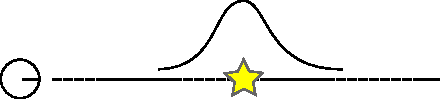
\includegraphics[width=0.6\columnwidth]{./images/simple_observation_model.pdf}
    \end{figure}    
\end{frame}

 \section{Extended Kalman Filter (EKF)}
 \begin{frame}
    \frametitle{Kalman Filter}
    \note{information taken from https://youtu.be/PiCC-SxWlH8}
   
    \begin{itemize}
    \item It is a Bayes Filter
    \item Everything is Gaussian
    \begin{equation*}
    p(x)=\det(2\pi\covariance)^{\frac{1}{2}} \exp\left(-\dfrac{1}{2} (x - \mu )^{\top} \inverse{\covariance} (x - \mu ) \right)
    \end{equation*}
   
    \item Optimal solutions for linear models and Gaussian distributions.
    \end{itemize}
   
    \begin{figure}[!h]
    \centering
    \subfloat[\scriptsize Gaussian Distribution in 1D]
    {
    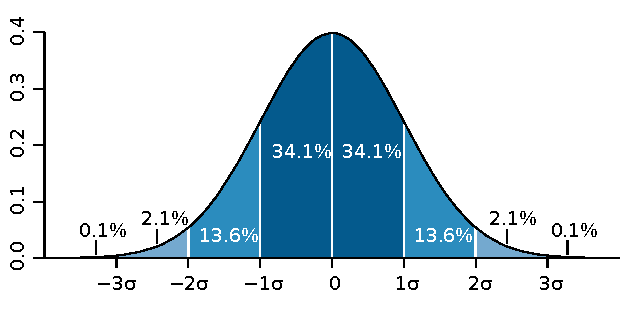
\includegraphics[width=0.3\columnwidth]{./images/standard_deviation_diagram.pdf}
    }
    \subfloat[\footnotesize 2D Gaussian Distribution]
    {
    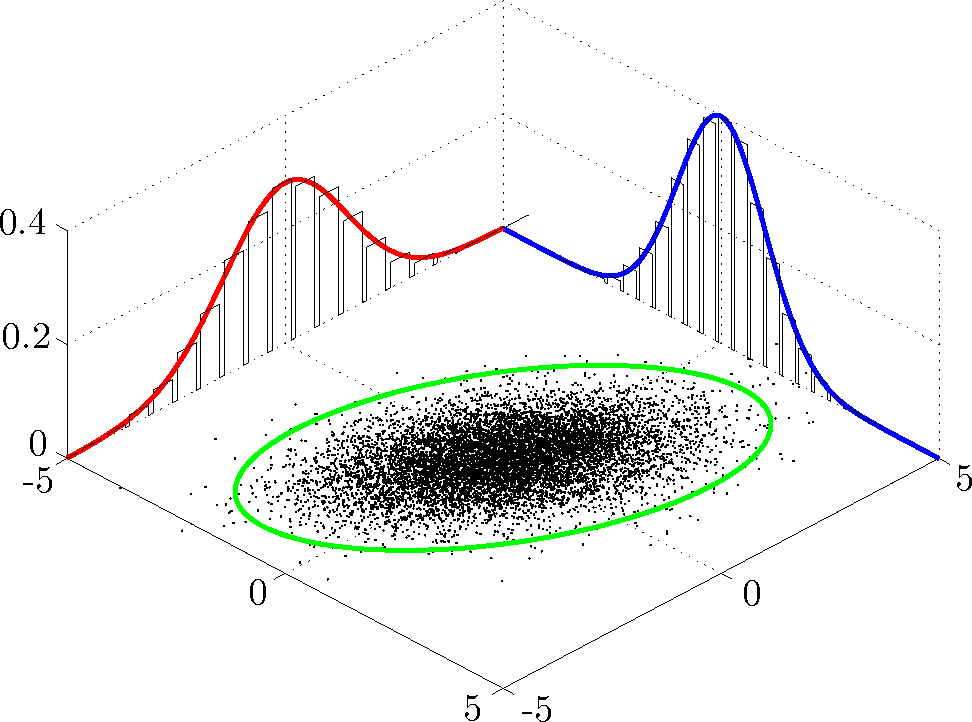
\includegraphics[width=0.3\columnwidth]{./images/multivariate_normal_sample.pdf}
    }
    \subfloat[\footnotesize 3D Gaussian Distribution]
    {
    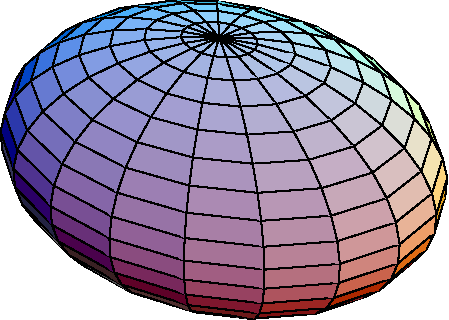
\includegraphics[width=0.25\columnwidth]{./images/ellipsoid.pdf}
    }
    \end{figure}
   \end{frame}
   
   
   \begin{frame}
    \frametitle{Kalman Filter Assumptions}
   \note{Information extracted from https://youtu.be/PiCC-SxWlH8}
   \note{Information extracted from https://www.youtube.com/watch?v=E-6paM\_Iwfc\&t=3442s}
   \small
   \begin{itemize}
   \item Noise and Gaussian Distributions
   \item Linear Motion and Observation Models
   \end{itemize}
   
   \begin{align*}
   \state_{t} &= \stateEvolutionMatrix_{t} \state_{t-1} + B_{t}\controlCommand_{t} + \motionModelNoise_{t}\\
   \observation_{t} &= C_{t} \state_{t} + \measurementModelNoise_{t}
   \end{align*}
   
   \begin{description}
   \item[$\stateEvolutionMatrix_{t}$] Matrix $(n \times n)$ describing how the state evolves from $t-1$ to $t$ without control commands or noise.
   
   \item[$B_{t}$] Matrix $(n \times l)$ describing how the control $\controlCommand_{t}$ changes the state from $t-1$ to $t$.
   
   \item[$C_{t}$] Matrix $(k \times n)$ describing how to map the state $\state_{t}$ to an observation $\observation_{t}$.
   
   \item[$\motionModelNoise_{t}$] Random variable representing the Gaussian noise of the motion model, assumed to be independent and normally distributed with mean zero and covariance $\motionParametersCovariance_{t}$.
   
   \item[$\measurementModelNoise_{t}$] Random variable representing the Gaussian noise of the {\bf observation model}, assumed to be independent and normally distributed with zero mean and covariance $\observationModelCovariance_{t}$.
   
   \end{description}
   
   \note{Kalman Filter requires that the noises be Gaussian and that the state result from a linear combination.}
   
   \note{Differential drive and Ackerman motion models are NOT linear models}
   \note{Observation models of a laser or a camera are also nonlinear.}
   \end{frame}
   
   \begin{frame}
   \frametitle{1D Kalman Filter}
   \note{Information taken from https://youtu.be/E-6paM_Iwfc}
   
   \begin{figure}[!h]
   \centering
   \subfloat[Initial Prediction]
   {
   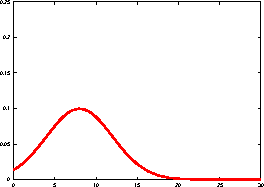
\includegraphics[width=0.3\columnwidth]{./images/kalman_filter_initial_prediction.pdf}
   }
   \subfloat[Measurement]
   { 
   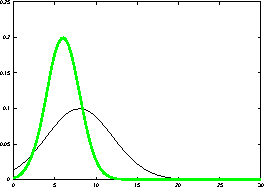
\includegraphics[width=0.3\columnwidth]{./images/kalman_filter_first_measurement.pdf}
    }
    \subfloat[Correction]
    {
    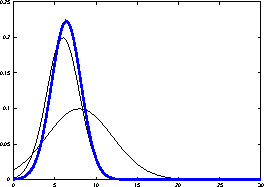
\includegraphics[width=0.3\columnwidth]{./images/kalman_filter_first_correction.pdf}
    }
    \end{figure}
   
   \end{frame}
   
   \begin{frame}
    \frametitle{1D Kalman Filter}
    \note{information taken from https://youtu.be/E-6paM_Iwfc}
   
    \begin{figure}[!h]
    \centering
    \subfloat[Motion Prediction]
    {
    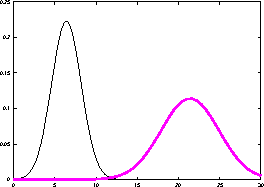
\includegraphics[width=0.3\columnwidth]{./images/kalman_filter_motion_prediction.pdf}
    }
    \subfloat[Second Measurement]
    {
    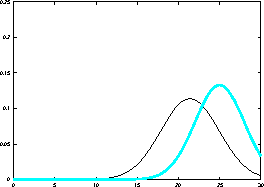
\includegraphics[width=0.3\columnwidth]{./images/kalman_filter_second_measurement.pdf}
    }
    \subfloat[Second Correction]
    {
    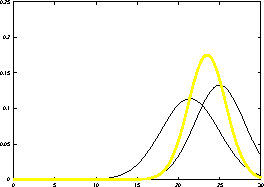
\includegraphics[width=0.3\columnwidth]{./images/kalman_filter_second_correction.pdf}
    }
    \end{figure}
   
\end{frame}

\begin{frame}
    \frametitle{Kalman Filter Assumptions}
    \note{Information taken from https://youtu.be/PiCC-SxWlH8}
    
    \begin{itemize}
    \item Noise and Gaussian Distributions
    \item Linear Motion and Observation Models
    \end{itemize}
    
    \begin{align*}
    \state_{t} &= A_{t} \state_{t-1} + B_{t}\controlCommand_{t} + \motionModelNoise_{t}\\
    \observation_{t} &= C_{t} \state_{t} + \measurementModelNoise_{t}
    \end{align*}
    \note{Kalman Filter requires that the noises be Gaussian and that the state result from a linear combination.}
    
    \centering
    \alert{What happens if these assumptions don't hold?}
    \note{Differential drive and Ackerman motion models are NOT linear models}
    \note{Observation models of a laser or a camera are not linear either.}
    \end{frame}
    
    \begin{frame}
    \frametitle{Non-linear Dynamical Systems}
    \note{Information taken from https://youtu.be/PiCC-SxWlH8}
    \begin{itemize}
    \item Real-life problems generally employ non-linear functions
    \end{itemize}
    
    % \begin{align*}
    % \state_{t} &= A_{t} \state_{t-1} + B_{t}\controlCommand_{t} + \motionModelNoise_{t}\\
    % \observation_{t} &= C_{t} \state_{t} + \measurementModelNoise_{t}
    % \end{align*}
    
    \begin{figure}[!h] 
    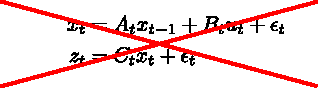
\includegraphics[width=0.4\columnwidth]{./images/kalman_filter_linear_equations_cross_out.pdf}
     \end{figure}
    
     \begin{align*}
     \state_{t} &= \motionModelFunction{\controlCommand_{t}, \state_{t-1}} + \motionModelNoise_{t}\\
     \observation_{t} &= \observationModelFunction{\state_{t}} + \measurementModelNoise_{t}
     \end{align*}
    
    \end{frame}
    
    \begin{frame}
     \frametitle{Linearity Assumption}
    
     \begin{figure}[!h]
     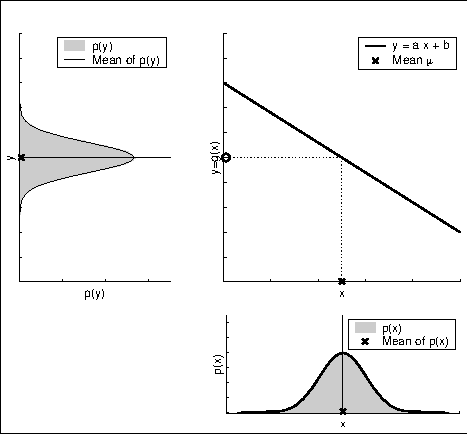
\includegraphics[width=0.5\columnwidth]{./images/linear_transformation_of_a_gaussian.pdf}
     \end{figure}
    \end{frame}
    
    \begin{frame}
    \frametitle{Nonlinear Function}
    
    \begin{figure}[!h]
    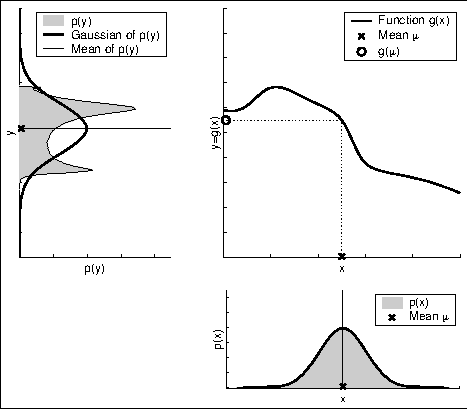
\includegraphics[width=0.5\columnwidth]{./images/nonlinear_transformation_of_a_gaussian.pdf}
    \end{figure}
    \end{frame}
    
    \begin{frame}
    \frametitle{Non-Gaussian Distributions}
    
    \note{Information taken from https://youtu.be/E-6paM\_Iwfc}
    
    \begin{itemize}
    \item Nonlinear functions lead to non-Gaussian distributions
    \item So, we can't apply the Kalman Filter!
    \end{itemize}
    
    \end{frame}
    
    \begin{frame}
     \frametitle{Linearization in EKF: First-order Taylor expansion}
    
     \note{Information taken from https://youtu.be/E-6paM\_Iwfc}
    
     \begin{itemize}
     \item Prediction:
     \begin{equation*}
     \motionModelFunction{\controlCommand_{t}, \state _{t-1}} \approx \motionModelFunction{\controlCommand_{t}, \mu _{t-1}} + \underbrace{\dfrac{\partial\motionModelFunction{\controlCommand_{t}, \mu _{t-1}}}{\partial\state _{t-1}}}_{\motionModelJacobian_{t}} (\state_{t-1} - \mu_{t-1})
     \end{equation*}
    
     \item Correction:
    
     \begin{equation*}
     \observationModelFunction{\state_{t}} \approx \observationModelFunction{\overline{\mu}_{t}} + \underbrace{\dfrac{\partial \observationModelFunction{\overline{\mu}_{t}}}{\partial \state_{t}}}_{\observationModelJacobian_{t}} (\state_{t} - \overline{\mu}_{t})
     \end{equation*}
    
     \end{itemize}
    
     $\motionModelJacobian_{t}$ and $\observationModelJacobian_{t}$ are called Jacobians.
    \end{frame}
    
    \begin{frame}
     \frametitle{Remembering Jacobians}
    
     \begin{itemize}
     \item In general it is a non-square matrix $m \times n$
     \item Given a vector function
    
     \begin{equation*}
     g(x) =
     \begin{bmatrix}
     g_{1}(x) \\
     g_{2}(x) \\
     \vdots \\
     gm(x)
     \end{bmatrix}
     \end{equation*}
    
     \item The Jacobian is defined as
     \begin{equation*}
     G_x =
     \begin{bmatrix}
     \dfrac{\partial g_{1}}{\partial x_{1}} & \dfrac{\partial g_{1}}{\partial x_{2}}& \dots & \dfrac{\partial g_{1}}{\partial x_{n}}\\
     \dfrac{\partial g_{2}}{\partial x_{1}} & \dfrac{\partial g_{2}}{\partial x_{2}}& \dots & \dfrac{\partial g_{2}}{\partial x_{n}}\\
     \vdots & \vdots& \vdots & \vdots\\
     \dfrac{\partial g_{m}}{\partial x_{1}} & \dfrac{\partial g_{m}}{\partial x_{2}}& \dots & \dfrac{\partial g_{m}}{\partial x_{n}}
     \end{bmatrix}
     \end{equation*}
     \end{itemize}
\end{frame}

\begin{frame}
    \frametitle{Remembering Jacobians}
    
    \begin{itemize}
    \item The Jacobian is the orientation of the tangent plane to a vector function at a given point
    \item The Jacobian is the generalization of the gradient of a scalar function
    \end{itemize}
    
    \begin{figure}[!h]
    \centering
    \subfloat[]
    {
    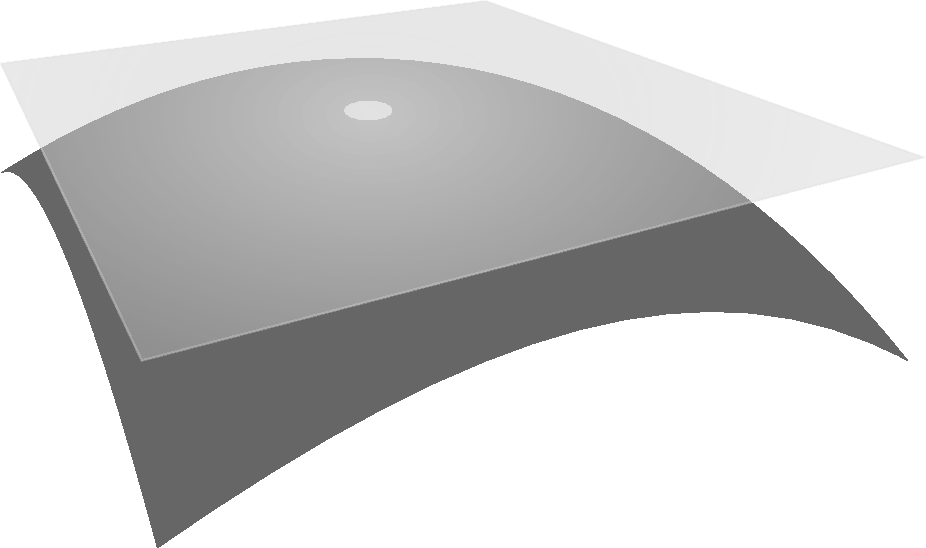
\includegraphics[valign=m,width=0.3\columnwidth]{./images/jacobian_tangent_plane.pdf}
    }
    \hspace{1cm} \subfloat[]
    {
    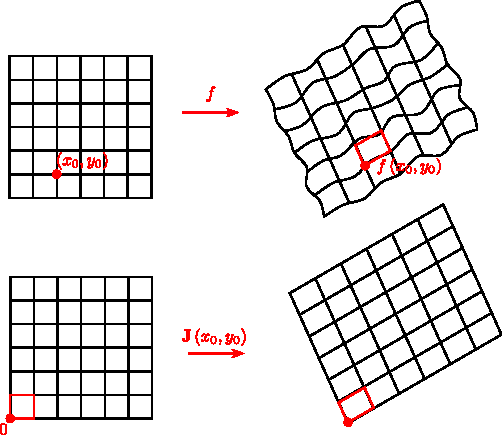
\includegraphics[valign=m,width=0.4\columnwidth]{./images/jacobian_local_linear_transform.pdf}
    }
    \end{figure}
    
    \begin{center}
    \end{center}
    
    \note{Info: https://angeloyeo.github.io/2020/07/24/Jacobian_en.html}
    
    \end{frame}
    
    
    \begin{frame}
     \frametitle{Linear Transformation}
    
     \begin{center}
     \movie[autostart,loop,poster]{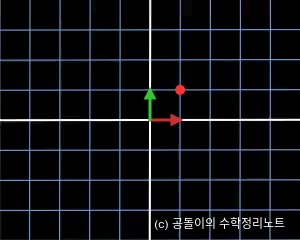
\includegraphics[width=0.6\columnwidth]{images/matrix_as_linear_transformation_video.jpg}}{videos/matrix_as_linear_transformation.mp4}
     \end{center}
    
     \note{Info: https://angeloyeo.github.io/2020/07/24/Jacobian_en.html}
    
    \end{frame}
    
    
    \begin{frame}
     \frametitle{Non-Linear Transformation}
    
     \begin{center}
     \movie[autostart,loop,poster]{
\includegraphics[width=0.5\columnwidth]{images/jacobian_nonlinear_transform_video.jpg}}{videos/jacobian_nonlinear_transform.mp4}
     \end{center}
    
     \note{Info: https://angeloyeo.github.io/2020/07/24/Jacobian_en.html}
    
    \end{frame}
    
    \begin{frame}
     \frametitle{Non-Linear (but Locally Linear) Transformation}
    
     \begin{center}
     \movie[autostart,loop,poster]{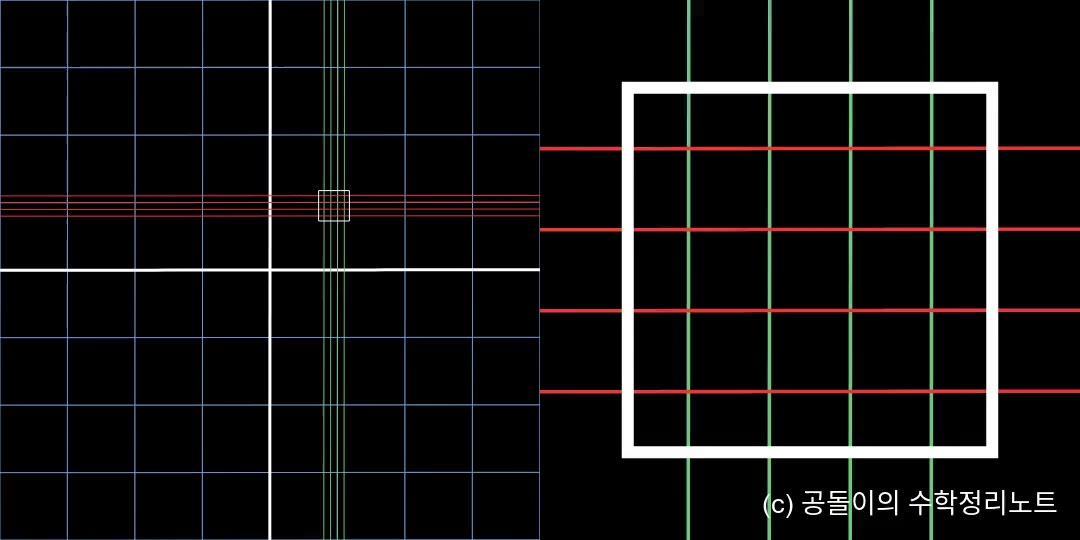
\includegraphics[width=\columnwidth]{images/jacobian_locally_linear_video.jpg}}{videos/jacobian_locally_linear.mp4}
     \end{center}
    
     \note{Info: https://angeloyeo.github.io/2020/07/24/Jacobian_en.html}
    
    \end{frame}
    
    
    \begin{frame}
     \frametitle{Linearization in EKF}
    
     \begin{figure}[!h]
     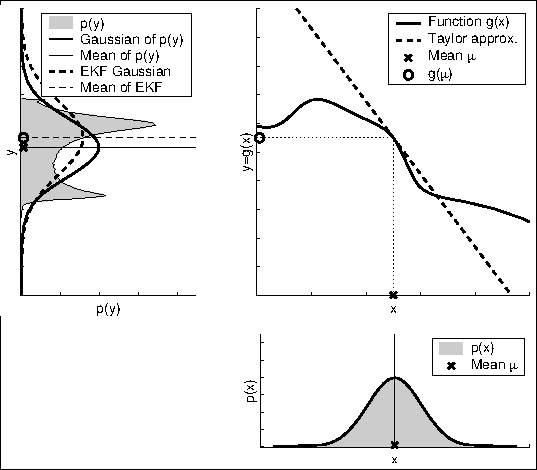
\includegraphics[width=0.5\columnwidth]{./images/linearization_applied_by_ekf.pdf}
     \end{figure}
    \end{frame}
    
    
    \begin{frame}
     \frametitle{Quality of Linearization in EKF}
    
     \begin{figure}[!h]
     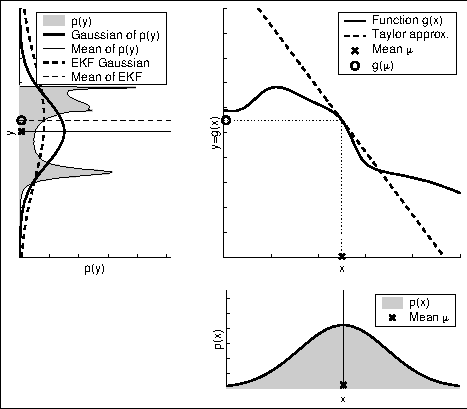
\includegraphics[width=0.5\columnwidth]{./images/dependency_approximation_quality_spread.pdf}
     \end{figure}
    \end{frame}
    
    \begin{frame}
     \frametitle{Quality of Linearization in EKF}
    
     \begin{figure}[!h]
    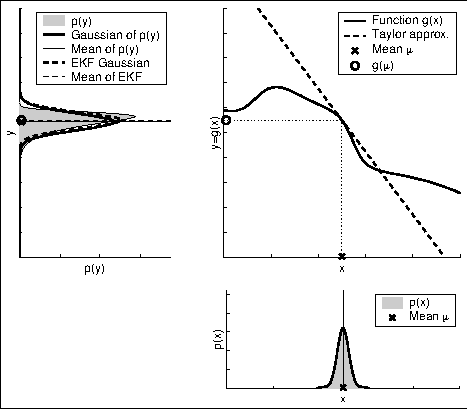
\includegraphics[width=0.5\columnwidth]{./images/dependency_approximation_quality_narrow.pdf}
    \end{figure}
    \end{frame}
    
    \begin{frame}
    \frametitle{Linearized Motion Model}
    \note{Information taken from https://youtu.be/PiCC-SxWlH8}
    
    \begin{itemize}
    \item Linearizing the model is given by:
    \begin{align*}
    p(\state_{t} | \controlCommand_{t}, \state _{t-1}) &\approx \det(2 \pi \motionParametersCovariance_{t})^{\frac{1}{2}}\\
     &\exp (-\dfrac{1}{2} (\state_{t} - \motionModelFunction{\controlCommand_{t}-\mu_{t-1}} - \motionModelJacobian_{t}(\state_{t-1}-\mu_{t-1}))^{\top}\\
     &\inverse{\motionParametersCovariance_{t}} (\state_{t} - \underbrace{\motionModelFunction{\controlCommand_{t},\mu_{t-1}} - \motionModelJacobian_{t} (\state_{t-1}-\mu_{t-1})}_{\text{model linearized}}))
    \end{align*}
    
    \item $\motionParametersCovariance_{t}$ describes motion noise
    \end{itemize}
    \end{frame}
    
    \begin{frame}
    \frametitle{Linearized observation model}
    \note{Information taken from https://youtu.be/PiCC-SxWlH8}
    
    \begin{itemize}
    \item Linearizing the model is given by:
    \begin{align*}
    p(\observation_{t} | \state_{t}) &\approx \det(2 \pi \observationModelCovariance_{t})^{\frac{1}{2}}\\
    &\exp (-\dfrac{1}{2} (\observation_{t} - \observationModelFunction{\overline{\mu_{t}}} - \observationModelJacobian_{t}(\state_{t} - \overline{\mu _{t}}))^{\top}\\
     &\inverse{\observationModelCovariance_{t}} (\observation_{t} - \underbrace{\observationModelFunction{\overline{\mu_{t}}} - \observationModelJacobian_{t} (\state_{t}-\overline{\mu_{t}})}_{\text{linearized model}}))
     \end{align*}
    
     \item $\observationModelCovariance_{t}$ describes the measurement noise
     \end{itemize}
    
    
\end{frame}

\begin{frame}
    \frametitle{Extended Kalman Filter Algorithm}
    \note{information taken from https://youtu.be/PiCC-SxWlH8}
   
    \begin{algorithmic}[1]
    \Procedure{ExtendedKalmanFilter}{$\mu_{t-1}, \covariance_{t-1}, \controlCommand_{t}, \observation_{t}$}
    \State $\overline{\mu}_{t} = \motionModelFunction{\controlCommand_{t}, \mu_{t-1}}$
    \State $\overline{\covariance}_{t} = \motionModelJacobian_{t} \covariance_{t-1} \motionModelJacobian_{t}^{\top}+\motionParametersCovariance_{t}$
    \Statex
    \State $\kalmanGain_{t} = \overline{\covariance}_{t} \observationModelJacobian_{t}^{\top} (\observationModelJacobian_{t} \overline{\covariance}_{t} \observationModelJacobian_{t} + \observationModelCovariance_{t})^{-1} $
    \State $\mu_{t} = \overline{\mu}_{t} + \kalmanGain_{t} (\observation_{t} - \observationModelFunction{\overline{\mu}_{t}})$
    \State $\covariance_{t} = (I - \kalmanGain_{t} \observationModelJacobian_{t}) \overline{\covariance}_{t}$
    \State \Return $\mu_{t}, \covariance_{t}$
    \EndProcedure
    \end{algorithmic}
   \end{frame}
   
   \section{EKF Location for feature-based map}
   
   \begin{frame}
    \frametitle{Odometry as controls}
    \note{information taken from https://youtu.be/PiCC-SxWlH8}
   
    \begin{figure}[!h]
    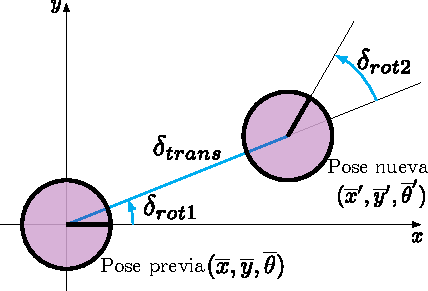
\includegraphics[width=0.6\columnwidth]{./images/odometry_as_controls.pdf}
    \end{figure}
   
    \begin{equation*}
    \controlCommand = (\delta _{rot1}, \delta _{trans}, \delta _{rot2})
    \end{equation*}
   
   \end{frame}
   
   \begin{frame}
    \frametitle{Motion model}
    \note{information taken from https://youtu.be/PiCC-SxWlH8}
   
    \begin{itemize}
    \item Motion Model Odometry
    \begin{equation*}
    \begin{bmatrix}
    x^{\prime} \\
    y^{\prime} \\
    \theta^{\prime}
    \end{bmatrix} =
    \underbrace{
    \begin{bmatrix}
    x \\
    and \\
    \theta
    \end{bmatrix} +
    \begin{bmatrix}
    \delta_{trans}\cos(\theta+\delta_{rot_{1}}) \\
    \delta_{trans}\sin(\theta+\delta_{rot_{1}}) \\
    \delta_{rot_{1}} + \delta_{rot_{2}}
    \end{bmatrix}
    }_{\motionModelFunction{\controlCommand_{t}, \state_{t-1}}} + \normalDistribution{0}{\motionParametersCovariance_{t}}
    \end{equation*}
    \item Linearization
    \begin{equation*}
    \motionModelFunction{\controlCommand_{t}, \state _{t-1}} \approx \motionModelFunction{\controlCommand_{t}, \mu _{t-1}} + \motionModelJacobian_{t}(\state _{t-1}-\mu _{t-1})
    \end{equation*}
    \end{itemize}
   
   \end{frame}
   
   \begin{frame}
    \frametitle{Jacobians of the motion model}
    \note{information taken from https://youtu.be/PiCC-SxWlH8}
    We calculate the Jacobian with respect to the state
    \begin{equation*}
    \motionModelJacobian_{t} = \dfrac{\delta\motionModelFunction{\controlCommand_{t},\mu _{t-1}}}{\delta \state _{t-1}} =
    \begin{bmatrix}
    \dfrac{\delta x^{\prime}}{\delta \mu _{t-1,x}} & \dfrac{\delta x^{\prime}}{\delta \mu _{t-1,y}} & \dfrac{\delta x^{\prime}}{\delta \mu _{t-1,\theta}}\\
    \dfrac{\delta y^{\prime}}{\delta \mu _{t-1,x}} & \dfrac{\delta y^{\prime}}{\delta \mu _{t-1,y}} & \dfrac{\delta y^{\prime}}{\delta \mu _{t-1,\theta}}\\
    \dfrac{\delta \theta^{\prime}}{\delta \mu _{t-1,x}} & \dfrac{\delta \theta^{\prime}}{\delta \mu _{t-1,y}} & \dfrac{\delta \theta^{\prime}}{\delta \mu _{t-1,\theta}}\\
    \end{bmatrix}
    \end{equation*}
   
    \begin{equation*}
    \motionModelJacobian_{t} =
    \begin{bmatrix}
    1 & 0 & -\delta_{trans} \sin(\theta + \delta_{rot_{1}})\\
    0 & 1 & \delta_{trans} \cos(\theta + \delta_{rot_{1}})\\
    0 & 0 & 1\\
    \end{bmatrix}
    \end{equation*}
\end{frame}

\begin{frame}
    \frametitle{Jacobians of the motion model}
    \note{information taken from https://youtu.be/PiCC-SxWlH8}
    
    We calculate the Jacobian with respect to the control command
    \begin{equation*}
    \motionModelJacobianControl{t} = \dfrac{\delta\motionModelFunction{\controlCommand_{t},\mu_{t-1}}}{\delta \controlCommand_{t}} =
    \begin{bmatrix}
    \dfrac{\delta x^{\prime}}{\delta \controlCommand_{t,\delta_{rot_{1}}}} & \dfrac{\delta x^{\prime}}{\delta \controlCommand_{t,\delta_{trans}}} & \dfrac{\delta x^{\prime}}{\delta \controlCommand_{t,\delta_{rot_{2}}}}\\
     \dfrac{\delta y^{\prime}}{\delta \controlCommand_{t,\delta _{rot_{1}}}} & \dfrac{\delta y^{\prime}}{\delta \controlCommand_{t,\delta _{trans}}} & \dfrac{\delta y^{\prime}}{\delta \controlCommand_{t,\delta _{rot_{2}}}}\\
     \dfrac{\delta \theta^{\prime}}{\delta \controlCommand_{t,\delta _{rot_{1}}}} & \dfrac{\delta \theta^{\prime}}{\delta \controlCommand_{t,\delta _{trans}}} & \dfrac{\delta \theta^{\prime}}{\delta \controlCommand_{t,\delta _{rot_{2}}}}
     \end{bmatrix}
     \end{equation*}
    
     \begin{equation*}
     \motionModelJacobianControl_{t} =
     \begin{bmatrix}
     -\delta_{trans} \sin(\theta + \delta _{rot_{1}}) & \cos(\theta + \delta _{rot_{1}}) & 0\\
     \delta _{trans} \cos(\theta + \delta _{rot_{1}}) & \sin(\theta + \delta _{rot _{1}}) & 0\\
     1 & 0 & 1\\
     \end{bmatrix}
     \end{equation*}
    \end{frame}
    
    \begin{frame}
     \frametitle{Observation model}
     \note{information taken from https://youtu.be/PiCC-SxWlH8}
     \begin{itemize}
     \item Range-bearing model
     \begin{equation*}
     \observation_{t}^{i} =
     \begin{bmatrix}
     r_{t}^{i}\\
     \phi_{t}^{i}
     \end{bmatrix} =
     \begin{bmatrix}
     \sqrt{(m_{j,x}-x)^{2} + (m_{j,y}-y)^{2}}\\
     \atantwo(m_{j,y}-y, m_{j,x}-x) -\theta
     \end{bmatrix}
     + \normalDistribution{0}{\observationModelCovariance_{t}}
     \end{equation*}
    
     \item Linearization
     \begin{equation*}
     \observationModelFunction{\state_{t}, m} \approx \observationModelFunction{\overline{\mu}_{t}} + \observationModelJacobian_{t}^{i}(\state_{t}-\overline{\mu}_{t})
     \end{equation*}
     \end{itemize}
    
    \end{frame}
    
    \begin{frame}
     \frametitle{Jacobians of the observation model}
     \note{information taken from https://youtu.be/PiCC-SxWlH8}
     We calculate the Jacobian with respect to the state
     \begin{equation*}
     \observationModelJacobian_{t} = \dfrac{\delta\observationModelFunction{\overline{\mu}_{t},m}}{\delta \state_{t}} =
     \begin{bmatrix}
     \dfrac{\delta r_{t}^{i}}{\delta \overline{\mu}_{t,x}} & \dfrac{\delta r_{t}^{i}}{\delta \overline{\mu}_{t,y}} & \dfrac{\delta r_{t}^{i}}{\delta \overline{\mu}_{t,\theta}}\\
     \dfrac{\delta \phi _{t}^{i}}{\delta \overline{\mu}_{t,x}} & \dfrac{\delta \phi _{t}^{i}}{\delta \overline{\mu}_{t,y}} & \dfrac{\delta \phi _{t}^{i}}{\delta \overline{\mu}_{t,\theta}}
     \end{bmatrix}
     \end{equation*}
    
     \begin{equation*}
     \observationModelJacobian_{t}^{i} =
     \begin{bmatrix}
     -\dfrac{m_{j,x} - \overline{\mu}_{t,x}}{\sqrt{q}} & -\dfrac{m_{j,y} - \overline{\mu}_{t,y}}{\sqrt{q}} & 0\\
     \dfrac{m_{j,y} - \overline{\mu}_{t,y}}{q} & -\dfrac{m_{j,x} - \overline{\mu}_{t,x}}{q} & -1
     \end{bmatrix}
     \end{equation*}
     where
     \begin{equation*}
     q = (m_{j,x}-\overline{\mu}_{t,x})^{2} + (m_{j,y}-\overline{\mu}_{t,y})^{2}
     \end{equation*}
\end{frame}

\begin{frame}
    \frametitle{Extended Kalman Filter Algorithm}
    \note{information taken from https://youtu.be/PiCC-SxWlH8}
    \footnotesize
    \begin{algorithmic}[1]
    \State ExtendedKalmanFilter({$\mu_{t-1}, \covariance_{t-1}, \controlCommand_{t}, \observation_{t}$, $c_{t}$, $m$})
    \State $\theta = \mu_{t-1,\theta}$
   
    \State $
    \motionModelJacobian_{t} =
    \begin{bmatrix}
    1 & 0 & -\delta_{trans} \sin(\theta + \delta_{rot_{1}})\\
    0 & 1 & \delta_{trans} \cos(\theta + \delta_{rot_{1}})\\
    0 & 0 & 1\\
    \end{bmatrix}
    $
    \State $
    \motionModelJacobianControl_{t} =
    \begin{bmatrix}
    -\delta_{trans} \sin(\theta + \delta _{rot_{1}}) & \cos(\theta + \delta _{rot_{1}}) & 0\\
    \delta _{trans} \cos(\theta + \delta _{rot_{1}}) & \sin(\theta + \delta _{rot _{1}}) & 0\\
    1 & 0 & 1\\
    \end{bmatrix}
    $
    \State $
    \motionModelCovariance_{t} =
    \begin{bmatrix}
    \alpha_{1}\delta^{2}_{rot_{1}} + \alpha_{2}\delta^{2}_{trans} & 0 & 0\\
    0 & \alpha_{3} \delta^{2}_{trans} + \alpha_{4} \left( \delta^{2}_{rot_{1}} + \delta^{2}_{rot_{2}} \right) & 0\\
    0 & 0 & \alpha_{1}\delta^{2}_{rot_{2}} + \alpha_{2}\delta^{2}_{trans}\\
    \end{bmatrix}
    $
    \State $\overline{\mu}_{t} = \mu_{t-1} +
    \begin{bmatrix}
    \delta_{trans}\cos(\theta+\delta_{rot_{1}}) \\
    \delta_{trans}\sin(\theta+\delta_{rot_{1}}) \\
    \delta_{rot_{1}} + \delta_{rot_{2}}
    \end{bmatrix}$
    \State $\overline{\covariance}_{t} = \motionModelJacobian_{t} \covariance_{t-1} \motionModelJacobian_{t}^{\top}+\motionModelJacobianControl_{t} \motionModelCovariance_{t} \motionModelJacobianControl_{t}^{\top}$
    \end{algorithmic}
    \vspace{1em}
    $M_{t}$ is a covariance that models the noise in the control commands.
    $\motionModelJacobianControl_{t} \motionModelCovariance_{t} \motionModelJacobianControl_{t}^{\top}$ refers to the uncertainty that is added due to noise in the control commands.
   
   \end{frame}
   
   \begin{frame}
   \frametitle{Prediction step}
   \note{Information taken from https://youtu.be/PiCC-SxWlH8}
   
   \begin{figure}[!h]
   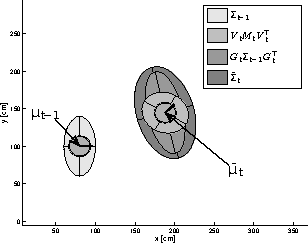
\includegraphics[width=0.5\columnwidth]{./images/ekf_prediction_step.pdf}
   \caption{Pose Prediction}
   \end{figure}
   
   \end{frame}
   
   \begin{frame}
   \frametitle{Extended Kalman Filter Algorithm}
   \note{Information taken from https://youtu.be/PiCC-SxWlH8}
   \footnotesize
   \begin{algorithmic}[1]
   \State
   $ \observationModelCovariance_{t} =
   \begin{bmatrix}
   \sigma_{r}^{2} & 0\\
   0 & \sigma_{\phi}^{2}
    \end{bmatrix}
    $
    \For {all observed features $z_{t}^{i} = (r_{t}^{i}, \phi_{t}^{i})^{\top}$}
   
    \State $ j = c_{t}^{i}$
    \State $ q = (m_{j,x}-\overline{\mu}_{t,x})^{2} + (m_{j,y}-\overline{\mu}_{t,y})^{2} $
    \State
    $ \hat{\observation}_{t}^{i} =
    \begin{bmatrix}
    \sqrt{q}\\
    \atantwo(m_{j,y}-\overline{\mu}_{t,y}, m_{j,x}-\overline{\mu}_{t,x}) - \overline{\mu}_{t,\theta}
    \end{bmatrix}
    $
    \State
    $ \observationModelJacobian_{t}^{i} =
    \begin{bmatrix}
    -\dfrac{m_{j,x} - \overline{\mu}_{t,x}}{\sqrt{q}} & -\dfrac{m_{j,y} - \overline{\mu}_{t,y}}{\sqrt{q}} & 0\\
    \dfrac{m_{j,y} - \overline{\mu}_{t,y}}{q} & -\dfrac{m_{j,x} - \overline{\mu}_{t,x}}{q} & -1
    \end{bmatrix}
    $
   
    \State $S_{t}^{i} = \observationModelJacobian_{t}^{i} \overline{\covariance}_{t} \observationModelJacobian_{t}^{i^{\top}} + \observationModelCovariance_{t} $
   
    \State $\kalmanGain_{t}^{i} = \overline{\covariance}_{t} {\observationModelJacobian_{t}^{i}}^{\top} S_{t}^{i^{-1}} $
    \State $\overline{\mu}_{t} = \overline{\mu}_{t} + \kalmanGain_{t}^{i}(\observation_{t} - \hat{\observation}_{t}^{i})$
    \State $\overline{\covariance}_{t} = (I - \kalmanGain_{t}^{i}\observationModelJacobian_{t}^{i})\overline{\covariance}_{t}$
   
    \EndFor
    \State $\mu_{t} = \overline{\mu}_{t}$
    \State $\covariance_{t} = \overline{\covariance}_{t}$
   
    \State \Return $\mu_{t}, \covariance_{t}$
    \end{algorithmic}
   
   
\end{frame}

\begin{frame}
    \frametitle{Measurement Prediction}
    \note{information taken from https://youtu.be/PiCC-SxWlH8}
    
    \begin{figure}[!h]
    \centering
    \subfloat[Pose Prediction]
    {
    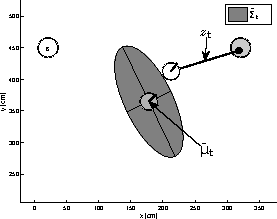
\includegraphics[width=0.45\columnwidth]{./images/ekf_pose_prediction.pdf}
    }
    \subfloat[Measurement Prediction]
    {
    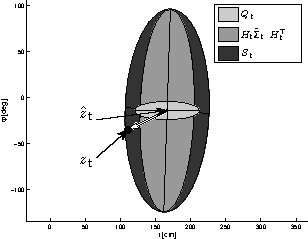
\includegraphics[width=0.45\columnwidth]{./images/ekf_measurement_prediction.pdf}
    }
    \end{figure}
    \footnotesize
    \begin{itemize}
    \item The robot's ground truth and the measurement are indicated by the white circle and the bold line, respectively.
    
    \item The white arrow indicates the \textbf{innovation} difference between observation and prediction of measurement. \end{itemize}
    
    \end{frame}
    
    \begin{frame}
    \frametitle{Correction step}
    \note{Information taken from https://youtu.be/PiCC-SxWlH8}
    
    \begin{figure}[!h]
    \centering
    \subfloat[Measurement Prediction]
    {
    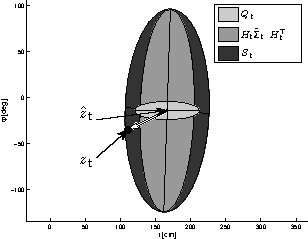
\includegraphics[width=0.45\columnwidth]{./images/ekf_measurement_prediction.pdf}
    }
    \subfloat[Measurement Correction]
    {
    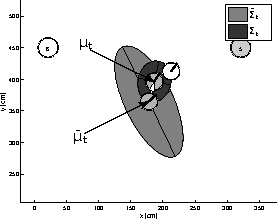
\includegraphics[width=0.45\columnwidth]{./images/ekf_measurement_correction.pdf}
    }
    \end{figure}
    
    \end{frame}
    
    \begin{frame}
    \frametitle{Example: EKF Localization 2D}
    \note{Information taken from the book Probabilistic Robotics}
    
    \begin{figure}[!h]
    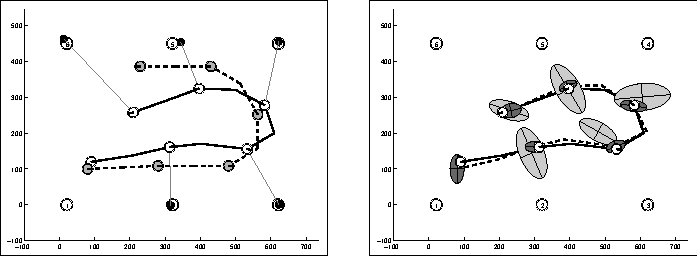
\includegraphics[width=\columnwidth]{./images/ekf_localization_example.pdf}
    \end{figure}
    
    The solid line is the ground truth. In the first graph, the dotted line is the odometry, and in the second graph, it is the estimate given by the EKF.
    
    \end{frame}
    
    \begin{frame}
    \frametitle{EKF Summary}
    \note{Information taken from https://youtu.be/PiCC-SxWlH8}
    
    \begin{itemize}
    \item It is an extension of the Kalman Filter
    \item A way to work with nonlinearities
    \item Performs local linearizations
    \item Works well in practice for moderately nonlinear cases
    \item Large uncertainties lead to increased error
    \end{itemize}
    
    \end{frame}
    
    \begin{frame}
    \frametitle{Extended Kalman Filter}
    
    \note{Information taken from:
    Cyrill Stachniss KF and EKF: https://youtu.be/E-6paM_Iwfc
    Chebrolu EKF Localization: https://youtu.be/PiCC-SxWlH8}
    
    \footnotesize 
    \url{https://automaticaddison.com/extended-kalman-filter-ekf-with-python-code-example/}
     \url{https://github.com/shangzhouye/EKF-SLAM-on-Turtlebot3}
    
     \url{https://github.com/ser94mor/sensor-fusion}
    
     \url{https://github.com/AtsushiSakai/PythonRobotics}
    
     It may be that the tp is just in python and the final tp is in ROS2.
    
     \url{https://github.com/debbynirwan/mcl}
    
    
\end{frame}


 \section{Particle Filter}
 \begin{frame}
    \frametitle{Particle Filter}
    \note{Information taken from Cyrill Stachniss's video https://youtu.be/MsYlueVDLI0}
    \footnotesize
    \begin{itemize}
    \item With EKF, we are restricted to Gaussian distributions.
    \item When we use EKF, we obtain a Gaussian distribution that describes where the robot is located.
    \item In Particle Filter, we use particles or hypotheses that describe where the robot could be.
    \item Instead of having a parametric form like EKF, which describes the probability distribution with the parameters mean $\mu$ and covariance $\covariance$, Partible Filter uses non-parametric samples as hypotheses about where the robot could be.
    
    \end{itemize}
    
    \begin{center}
    \movie[loop]{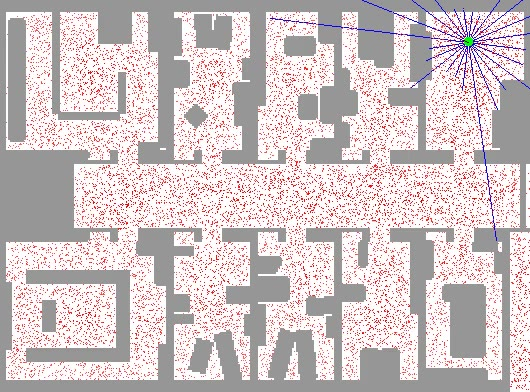
\includegraphics[width=0.4\columnwidth]{images/particle_filter/particle_filter_video.jpg}}{videos/particle_filter.mp4}
    \end{center}
    
    \note{Video taken from https://rse-lab.cs.washington.edu/projects/mcl/animations/global-floor.gif}
    
    \end{frame}
    
    \begin{frame}
    \frametitle{Approximation of a Function}
    \note{Information taken from Cyrill Stachniss's video https://youtu.be/MsYlueVDLI0}
    \footnotesize
    
    \begin{itemize}
    \item Objective: To be able to estimate any \textbf{arbitrary probability distribution}.
    \end{itemize}
    
    \begin{center}
    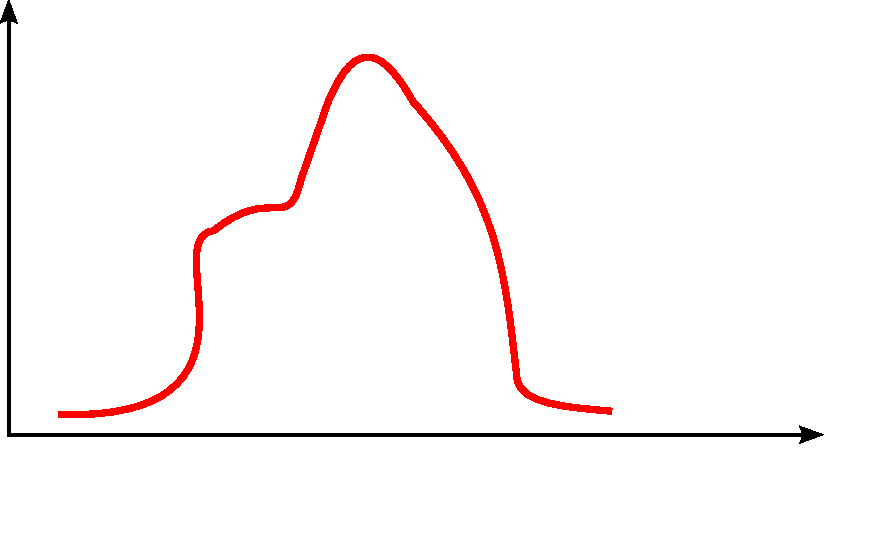
\includegraphics[width=0.5\columnwidth]{./images/particle_filter/arbitrary_distribution.pdf}
    \end{center}
    
    \end{frame}
    
    \begin{frame}
    \frametitle{Using Samples (Particles)}
    \note{Information taken from Cyrill Stachniss's video https://youtu.be/MsYlueVDLI0}
    \footnotesize
    \begin{itemize}
    \item \textbf{Multiple samples} to represent an arbitrary probability distribution
    \item Samples are more clustered in some areas and less so in others. The number of particles per unit area describes how likely it is that the robot is in that area.
    \item Each sample accumulates a bit of "probability mass."
    \item Samples can be viewed as an approximation to the probability density function (pdf).
    \item To obtain the PDF, you must integrate over a certain area to obtain the mathematical probability that the robot is in that area.
    \end{itemize}
    
    \begin{center}
    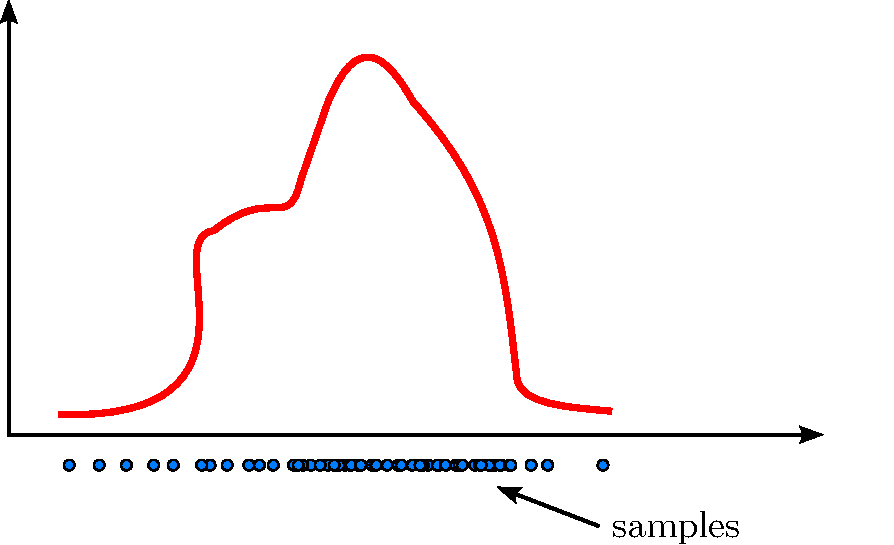
\includegraphics[width=0.5\columnwidth]{./images/particle_filter/arbitrary_distribution_samples.pdf}
    \end{center}
    
    \end{frame}
    
    \begin{frame}
    \frametitle{Using Weighted Samples}
    \note{Information taken from Cyrill Stachniss's video https://youtu.be/MsYlueVDLI0}
    \footnotesize
    \begin{itemize}
    \item \textbf{Multiple Weighted Samples} to Represent an Arbitrary Probability Distribution
    \item We can reduce the number of samples we need by adding weights to each sample.
    \item The more weight a sample has, the more probability mass there is in that region.
    \item The weights of all the particles together must sum to 1.
    \item Initially, we could add a uniform weight to each sample. For example, if we have $n$ samples, then each sample has weight $\frac{1}{n}$
    \end{itemize}
    
    \begin{center}
    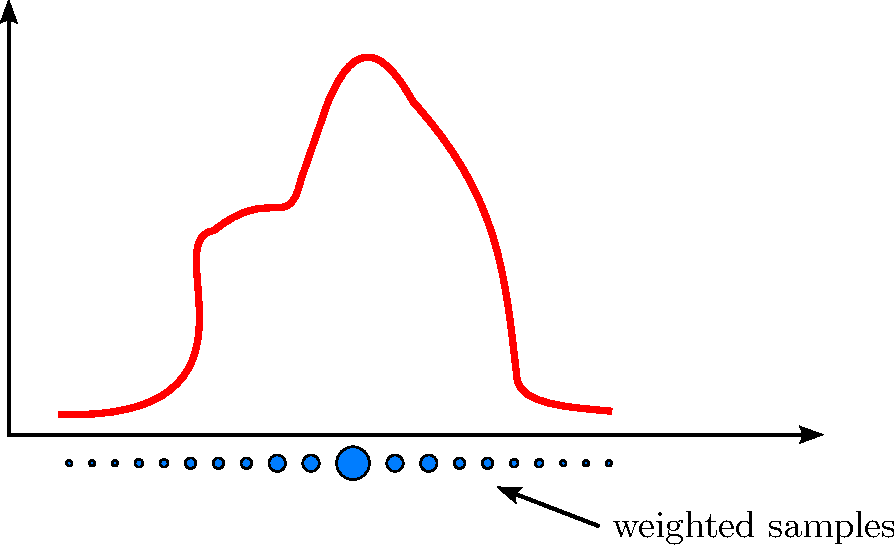
\includegraphics[width=0.5\columnwidth]{./images/particle_filter/arbitrary_distribution_weighted_samples.pdf}
    \end{center}
    
    \end{frame}
    
    \begin{frame}
    \frametitle{Particle Filter}
    \note{Information taken from Cyrill Stachniss's video https://youtu.be/MsYlueVDLI0}
    
    \footnotesize
    \begin{itemize}
    \item Note that this is an approximation of the pdf.
    \item It is important to have a sufficient number of samples to adequately represent the pdf.
    \end{itemize}
    
    
    \end{frame}
    
    
    \begin{frame}
     \frametitle{Material for Particle Filter}
    
     \begin{itemize}
     \item Information extracted from Video by Cyrill Stachniss https://youtu.be/MsYlueVDLI0
     \item https://rse-lab.cs.washington.edu/projects/mcl/
     \end{itemize}
    
    \end{frame}
    
    
    \begin{frame}
     \frametitle{TODO}
     \note{Information taken from Cyrill Stachniss Video https://youtu.be/MsYlueVDLI0}
     \note{https://rse-lab.cs.washington.edu/projects/mcl/}
    
     \TODO{USE THE SEMINAR SLIDE}
    
\end{frame}

 \section{Bibliography}
 \begin{frame}
	\frametitle{Bibliography}
   
    Static state binary Bayes filter:
    
    Capítulo 4.2 de \cite{thrun2005probabilistic}
    
    Occupancy Grid Mapping:
    
    Capítulo 9.1 y 9.2 de \cite{thrun2005probabilistic}
	
	\printbibliography
	
\end{frame}

 % Programming a robotic car seminar slides
 %\section{Medición}

\begin{frame}{Belief luego de sensar}
    \begin{block}{Ejemplo}
        \begin{itemize}
            \item Un mundo constituido por cinco celdas $x_{i}$ donde $i = 1, \dots ,5$
            \item Las celdas $x_{2}$ y $x_{3}$ son rojas, y el resto verdes.
            \item Inicialmente el robot desconoce su posición
            \item La probabilidad de que el robot sense correctamente  esta dada por la siguiente distribución de probabilidades:
            
            \begin{displaymath}
                P(sensa \ color | x_{i} = color) = 0.6
            \end{displaymath}
            \begin{displaymath}
                P(sensa \ \neg color | x_{i} = color) = 0.2
            \end{displaymath}
            
            Observar que no es una distribución de probabilidad correcta ya que la suma debe ser $1$.
            
        \end{itemize}
        
    \end{block}
    
    \begin{center}
        \includegraphics<1>[height=1.0cm]{./images/uniform_five_cells.png}
    \end{center}
    
\end{frame}

\begin{frame}{Belief luego de sensar}
    
    Si el robot \alert{sensa rojo}, ?`Cuál es su Posterior belief?
    
    \begin{center}
        \includegraphics<1>[height=3.5cm]{./images/inaccurate_sensing_quiz.png}
    \end{center}
\end{frame}

\begin{frame}{Belief luego de sensar}
    
    Si el robot \alert{sensa rojo}, ?`Cuál es su Posterior belief?
    
    \begin{center}
        \includegraphics<1>[height=3.5cm]{./images/inaccurate_sensing_solution.png}
    \end{center}
    \begin{footnotesize}
        \begin{displaymath}
            P(x_{i} = rojo | sensa \ rojo) = P(sensa \ rojo | x_{i} = rojo) P(x_{i}) = 0.2 \times 0.6 = 0.12
        \end{displaymath}
        \begin{displaymath}
            P(x_{i} = verde | sensa \ rojo) = P(sensa \ rojo | x_{i} = verde) P(x_{i}) = 0.2 \times 0.2 = 0.04
        \end{displaymath}
    \end{footnotesize}
    
\end{frame}

\begin{frame}{Belief luego de sensar}
    \begin{displaymath}
        P(x_{i} = rojo | sensa \ rojo) = 0.12
    \end{displaymath}
    \begin{displaymath}
        P(x_{i} = verde | sensa \ rojo) = 0.04
    \end{displaymath}
    
    Observar que estamos ante una distribución de probabilidades formalmente incorrecta dado que la suma: 
    \begin{displaymath}
        \sum_{i=1}^{5} P(x_{i}) = 0.04 + 0.12 + 0.12 + 0.04 + 0.04 = 0.36
    \end{displaymath}
    
    
    Si normalizamos la distribución, queda:
    
    \begin{displaymath}
        P(x_{i} = rojo| sensa \ rojo) = \dfrac{0.12}{0.36} = \dfrac{1}{3}
    \end{displaymath}
    \begin{displaymath}
        P(x_{i} = verde| sensa \ rojo) = \dfrac{0.04}{0.36} = \dfrac{1}{9}
    \end{displaymath}
    
    En general, $P(x_{i}|z)$ es la distribución Posterior belief del lugar $x_{i}$ dada la medición $z$.
\end{frame}


\begin{frame}{Regla de Bayes}
    
    Notar que cuando el robot sensa no hace otra cosa que aplicar la Regla Bayes:
    
    \begin{block}{Regla de Bayes}
        \begin{displaymath}
            P(x_{i} | z) = \dfrac{P(z | x_{i})P(x_{i})} {P(z)} 
        \end{displaymath}
        $P(x_{i} | z)$ : probabilidad a Posteriori (Posterior Belief) \\
        $P(z | x_{i})$ : probabilidad de Medición \\
        $P(x_{i})$ : probabilidad a Priori \\
        $P(z)$ : término de Normalización
    \end{block}
    
\end{frame}

\section{Motricidad}
\begin{frame}{Belief luego del movimiento}
    \begin{block}{Ejemplo (continuación)}
        \begin{itemize}
            \item Un mundo \alert{cíclico} constituido por cinco celdas $x_{i}$ donde $i = 1, \dots ,5$
            \item La distribución de probabilidad a priori esta determinada por:
            \begin{displaymath}
                P(x_{1}) = P(x_{4}) = P(x_{5}) = \dfrac{1}{9}
            \end{displaymath}
            \begin{displaymath}
                P(x_{2}) = P(x_{3}) = \dfrac{1}{3}    
            \end{displaymath}
        \end{itemize}
    \end{block}
    
\end{frame}

\begin{frame}{Belief luego del movimiento}
    Si el robot tiene una \alert{motricidad exacta} y desea moverse \alert{una} celda a la derecha, ?`Cuál es su Posterior belief?
    
    \begin{center}
        \includegraphics<1>[height=3.5cm]{./images/exact_motion_quiz.png}
    \end{center}
    
\end{frame}

\begin{frame}{Belief luego del movimiento}
    Si el robot tiene una \alert{motricidad exacta} y desea moverse \alert{una} celda a la derecha, ?`Cuál es su Posterior belief?
    
    \begin{center}
        \includegraphics<1>[height=3.5cm]{./images/exact_motion_solution.png}
    \end{center}
    
\end{frame}

\begin{frame}{Belief luego del movimiento}
    Suponiendo ahora que el robot desea moverse \alert{dos} celdas a la derecha y tiene una \alert{motricidad inexacta} con la siguiente distribución de probabilidad:
    \begin{columns}[t]
        \begin{column}{5cm}
            \begin{displaymath}
                P(x_{i+2}| x_{i}) = 0.8
            \end{displaymath}
            \begin{displaymath}
                P(x_{i+1}| x_{i}) = 0.1
            \end{displaymath}
            \begin{displaymath}
                P(x_{i+3}| x_{i}) = 0.1
            \end{displaymath}
        \end{column}
        \begin{column}{5cm}
            \begin{center}
                \includegraphics<1>[height=1.8cm]{./images/inexact_motion.png}
            \end{center}
        \end{column}
    \end{columns}
\end{frame}

\begin{frame}{Belief luego del movimiento}
    
    Si el robot conoce exactamente cuál es su posición inicial, ?`Cuál es su Posterior belief?
    
    \begin{columns}[t]
        \begin{column}{5cm}
            \begin{center}
                \includegraphics<1>[height=2.0cm]            {./images/inexact_motion_initial_pose_quiz.png}
            \end{center}
        \end{column}
        \begin{column}{5cm}
            \begin{center}
                \includegraphics<1>[height=1.8cm]{./images/inexact_motion.png}
            \end{center}
        \end{column}
    \end{columns}
\end{frame}

\begin{frame}{Belief luego del movimiento}
    
    Si el robot conoce exactamente cuál es su posición inicial, ?`Cuál es su Posterior belief?
    
    \begin{columns}[t]
        \begin{column}{5cm}
            \begin{center}
                \includegraphics<1>[height=2cm]            {./images/inexact_motion_initial_pose_solution.png}
            \end{center}
        \end{column}
        \begin{column}{5cm}
            \begin{center}
                \includegraphics<1>[height=1.8cm]{./images/inexact_motion.png}
            \end{center}
        \end{column}
    \end{columns}
\end{frame}

\begin{frame}{Belief luego del movimiento}
    Si el robot tiene como distribución inicial que se encuentra en las celdas $x_{2}$ y $x_{4}$ con igual probabilidad, formalmente,
    \begin{displaymath}
        P(x_{2}) = P(x_{4}) = 0.5
    \end{displaymath}
    ?`Cuál es su Posterior belief?
    
    \begin{columns}[t]
        \begin{column}{5cm}
            \begin{center}
                \includegraphics<1>[height=2cm]{./images/inexact_motion_quiz.png}
            \end{center}
        \end{column}
        \begin{column}{5cm}
            \begin{center}
                \includegraphics<1>[height=1.8cm]{./images/inexact_motion.png}
            \end{center}
        \end{column}
    \end{columns}
\end{frame}

\begin{frame}{Belief luego del movimiento}
    
    Si el robot tiene como distribución inicial que se encuentra en las celdas $x_{2}$ y $x_{4}$ con igual probabilidad, formalmente,
    \begin{displaymath}
        P(x_{2}) = P(x_{4}) = 0.5
    \end{displaymath}
    ?`Cuál es su Posterior belief?
    
    \begin{columns}[t]
        \begin{column}{5cm}
            \begin{center}
                \includegraphics<1>[height=2cm]{./images/inexact_motion_solution.png}
            \end{center}
        \end{column}
        \begin{column}{5cm}
            \begin{center}
                \includegraphics<1>[height=1.8cm]{./images/inexact_motion.png}
            \end{center}
        \end{column}
    \end{columns}
    \begin{small}
        $P(x_{1}) = P(x_{4}) P(x_{1}|x_{4}) = 0.5 \times 0.8 = 0.4$ \\
        $P(x_{2}) = P(x_{4}) P(x_{2}|x_{4}) = 0.5 \times 0.1 = 0.05$ \\
        $P(x_{3}) = P(x_{2}) P(x_{3}|x_{2}) = 0.5 \times 0.1 = 0.05$ \\    
        $P(x_{4}) = P(x_{2}) P(x_{4}|x_{2}) = 0.5 \times 0.8 = 0.4$ \\    
        $P(x_{5}) = P(x_{2}) {\color{red} P(x_{5}|x_{2})} + P(x_{4}) {\color{green} P(x_{5}|x_{4})} = 0.5 \times {\color{red} 0.1} + 0.5 \times {\color{green} 0.1} = 0.1$    
    \end{small}
\end{frame}

\section{Sensar y Mover}
\begin{frame}{Ciclo de sensar y mover}
    Localización no es más que la iteración de sensar y mover.
    \begin{center}
        \includegraphics<1>[height=2.5cm]{./images/sens_and_move.pdf}
    \end{center}
    
    \begin{block}{Entropía}
        Medida de información que tiene la distribución
        \begin{displaymath}
            - \sum P(x_{i}) \log P(x_{i})
        \end{displaymath}
        
        En otras palabras, la entropía expresa la información que un robot recibe luego de ejecutar una acción específica.
    \end{block}
    
\end{frame}


\begin{frame}{Definición formal de localización}
    
    \begin{block}{Medición}
        \begin{displaymath}
            \Bar{P}(x_{i}|z) \leftarrow P(z|x_{i}) P(x_{i})
        \end{displaymath}
        \begin{displaymath}
            \alpha \leftarrow \sum \Bar{P}(x_{i}|z)
        \end{displaymath}
        \begin{displaymath}
            P(x_{i}|z) \leftarrow \frac{1}{\alpha} \Bar{P}(x_{i}|z)
        \end{displaymath}
        
    \end{block}
    
\end{frame}

\begin{frame}{Definición formal de localización}
    
    Sea $P(x_{i}^{t})$ la probabilidad de estar en el punto $x_{i}$ luego del movimiento del robot
    
    \begin{block}{Motricidad}
        
        \begin{displaymath}
            P(x_{i}^{t}) = \sum_{j} P(x_{j}^{t-1}) P(x_{i}|x_{j})
        \end{displaymath}
        
    \end{block}
    
    La probabilidad de estar en $x_{i}$ se calcula a través de todos los lugares de los que podríamos haber venido
    
    Observar que la expresión anterior no es otra cosa que el Teorema de Probabilidad total.
    
    \begin{block}{Teorema de Probabilidad Total}
        
        \begin{displaymath}
            P(A) = \sum_{B}^{}P(A|B) P(B)
        \end{displaymath}
        
    \end{block}
    
\end{frame}

\end{document}